\documentclass{beamer}
\usepackage{mathptmx}
\usepackage[scaled=0.9]{helvet}
\usepackage{courier}
\usetheme{CambridgeUS}
\usepackage{textpos}
\usepackage{calc}
\graphicspath{{figures/}}




\title[Biospytial: a Graph Based Engine] % (optional, only for long titles)
{Introducing {\em Biospytial} }
\subtitle{An Open Source graph-based computing framework for managing and modeling spatial ecological data}
\author[Juan Escamilla Molgora] % (optional, for multiple authors)
{Juan Escamilla Molgora~\inst{1} ~\inst{2}}
\institute[Lancaster University] % (optional)
{
  \inst{1}%
	Lancaster Environment Center
  \and
  \inst{2}%
  Data Science Institute
}
\date[SPAT2017] % (optional)
{Spatial Statistics Conference, 2017}
\subject{Computer Science}




% position the logo
\addtobeamertemplate{frametitle}{}{%
\begin{textblock*}{\paperwidth}(1cm,1cm)

\includegraphics[height=1cm,width=1cm,keepaspectratio]{cat.jpeg}
\end{textblock*}}


\begin{document}
\begin{frame}
\titlepage
\end{frame}

\section{Motivations}

\begin{frame}
		\frametitle{Why are ecosystems important?}
		\begin{exampleblock}{Support}			
				\begin{figure}				
				\centering
		    	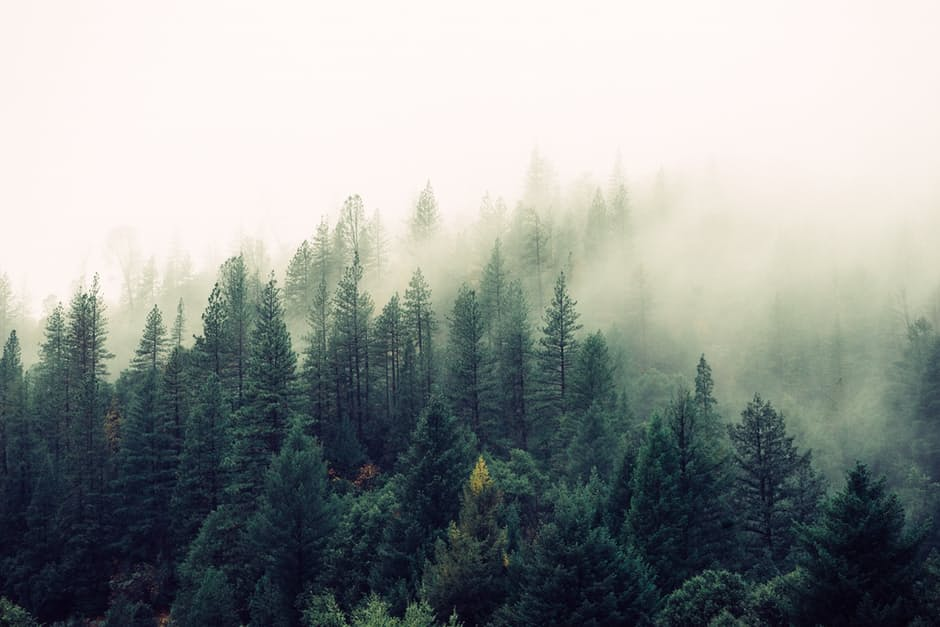
\includegraphics[height=0.7\textheight,width=\textwidth]{forest1.jpeg}		    	    
				\caption{Primary production}
		    	\end{figure}
		\end{exampleblock}
	\end{frame}

	\begin{frame}
		\frametitle{Why are ecosystems important?}
		\begin{exampleblock}{Support}			
				\begin{figure}				
				\centering
		    	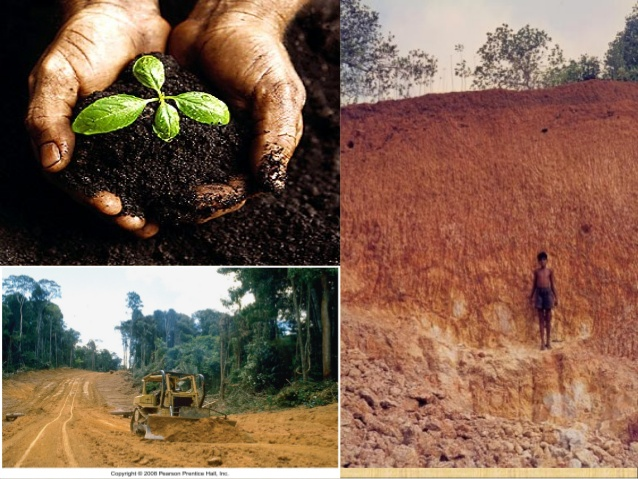
\includegraphics[height=0.7\textheight,width=\textwidth]{soil.jpg}		    	    
				\caption{Soil production}
		    	\end{figure}
		\end{exampleblock}
	\end{frame}

	\begin{frame}
		\frametitle{We drink water and breathe air}
		\begin{block}{Provisioning}
				\begin{figure}				
				\centering
		    	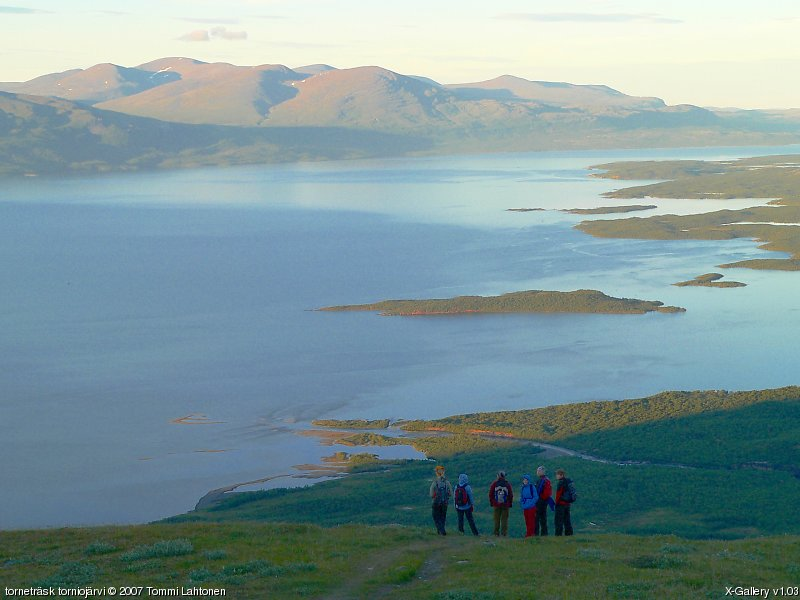
\includegraphics[height=0.7\textheight,width=\textwidth]{tornetrask.jpg}		    	    
				\caption{Water cycle and purification}
		    	\end{figure}
		\end{block}
	\end{frame}

	\begin{frame}
		\frametitle{We eat}
		\begin{block}{Provisioning}
				\begin{figure}				
				\centering
		    	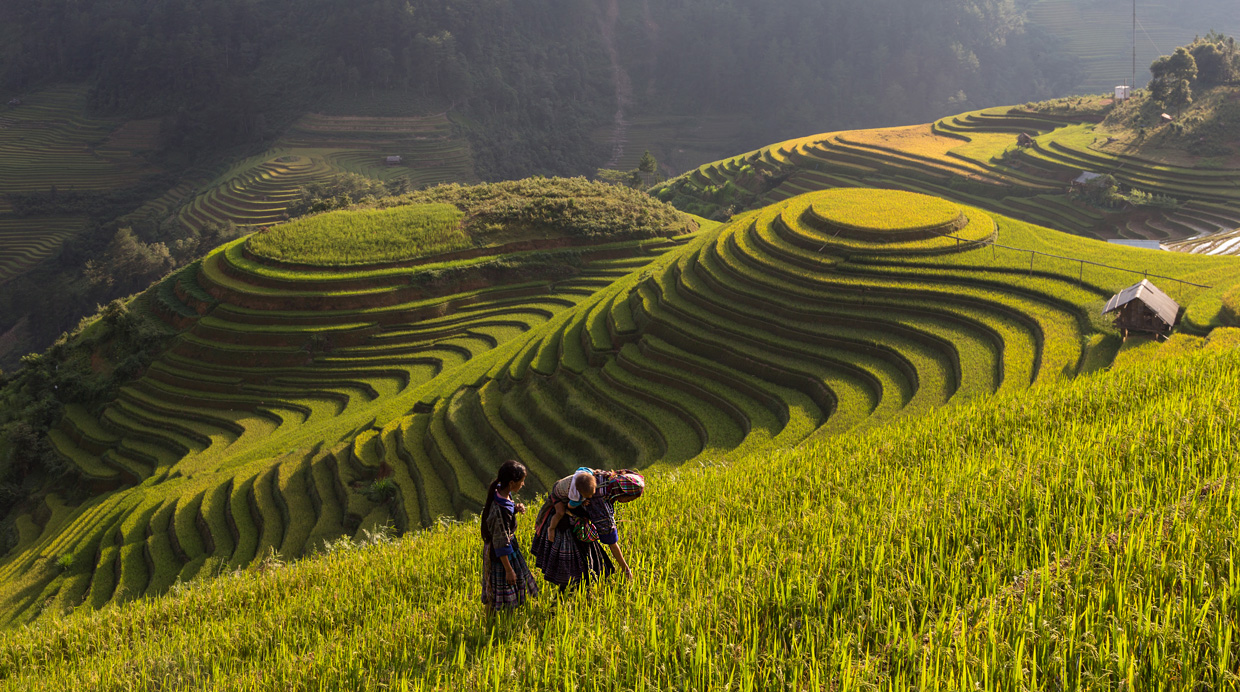
\includegraphics[height=0.7\textheight,width=\textwidth]{food.jpg}		    	    
				\caption{Food supply}
		    	\end{figure}
		\end{block}
	\end{frame}


	\begin{frame}
		\frametitle{Self-regulating systems}
		\begin{block}{Regulating Services}
				\begin{figure}				
				\centering
		    	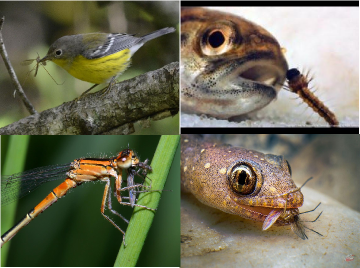
\includegraphics[height=0.7\textheight,width=\textwidth]{em.png}		    	    
				\caption{Disease regulator }
		    	\end{figure}
		\end{block}
	\end{frame}

	\begin{frame}
		\frametitle{}
		\begin{block}{Regulating services}
				\begin{figure}				
				\centering
		    	\includegraphics<1>[height=0.7\textheight,width=\textwidth]{reg2.jpg}
		    	\includegraphics<2>[height=0.7\textheight,width=\textwidth]{reg1.jpeg}		    	    
				\caption{Energy and salt concentration }
		    	\end{figure}
		\end{block}
	\end{frame}


\subsection{Why modelling?}
	\begin{frame}
		\frametitle{Why model them ?}
		\begin{block}{The environment changes}
				\begin{figure}				
				\centering
		    	\includegraphics<1>[height=0.6\textheight,width=\textwidth]{deforest1.png}	    	    
				\caption{ Landsat 5 images from June 24, 1984, and August 6, 2011. (U.S. Department of the Interior | U.S. Geological Survey)  }
		    	\end{figure}
		\end{block}
	\end{frame}

	\begin{frame}
		\frametitle{Why model them ?}
		\begin{block}{Climate Change Mitigation and Response}
				\begin{figure}				
\centering
		    	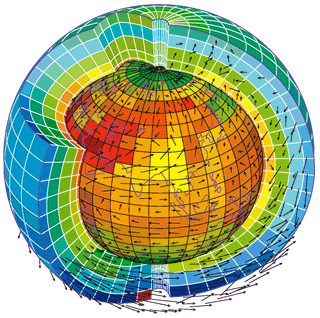
\includegraphics[width=0.4\textwidth]{ESM.png}
		    	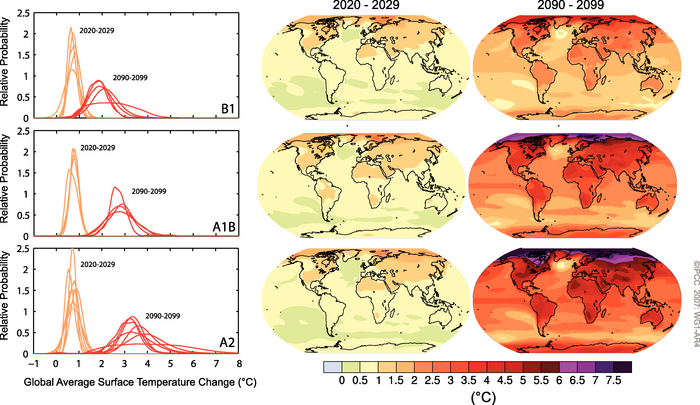
\includegraphics[width=0.6\textwidth]{ch1.png}		    	    
				\caption{Earth System Models ((L. Fairhead /LMD-CNRS) and IPCC, 2007)}
		    	\end{figure}
		\end{block}
	\end{frame}

	\begin{frame}
		\frametitle{Main question is ...}

				\begin{columns}
					\begin{column}{0.6\textwidth}
						\begin{block}{Spatial regression of ecological networks}						
						\begin{itemize}
						\item<1> {\em Find the underlying process that shapes the "species"assemblages.}
						\item<2> Infer the probability of assemblages of taxa for a given location.
						\end{itemize}										
					    \end{block}		
					\end{column}
				
			\begin{column}{0.5\textwidth}
			\centering
		    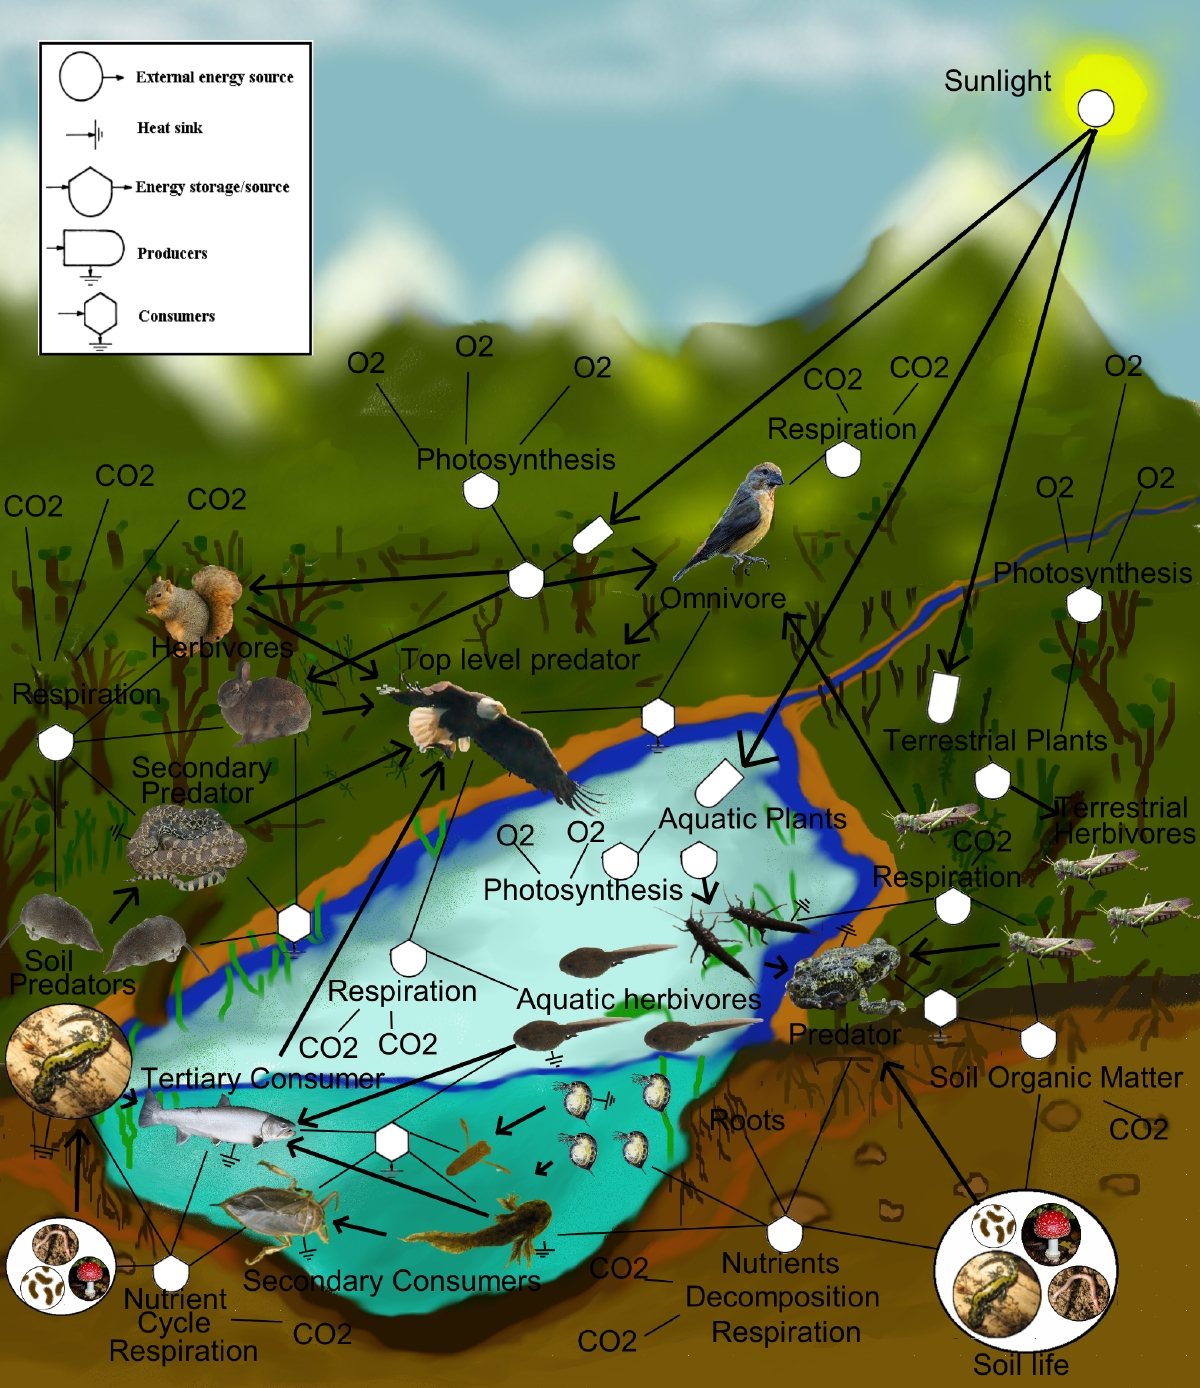
\includegraphics[scale=0.6]{/home/juan/Research/proposals/FoodWeb.jpg}		
		    \end{column}    	    
		\end{columns}
	\end{frame}




\section{Graph based Engine}
\subsection{Architecture}
\begin{frame}{Services and Modules}
Put here diagram paper1
\centering
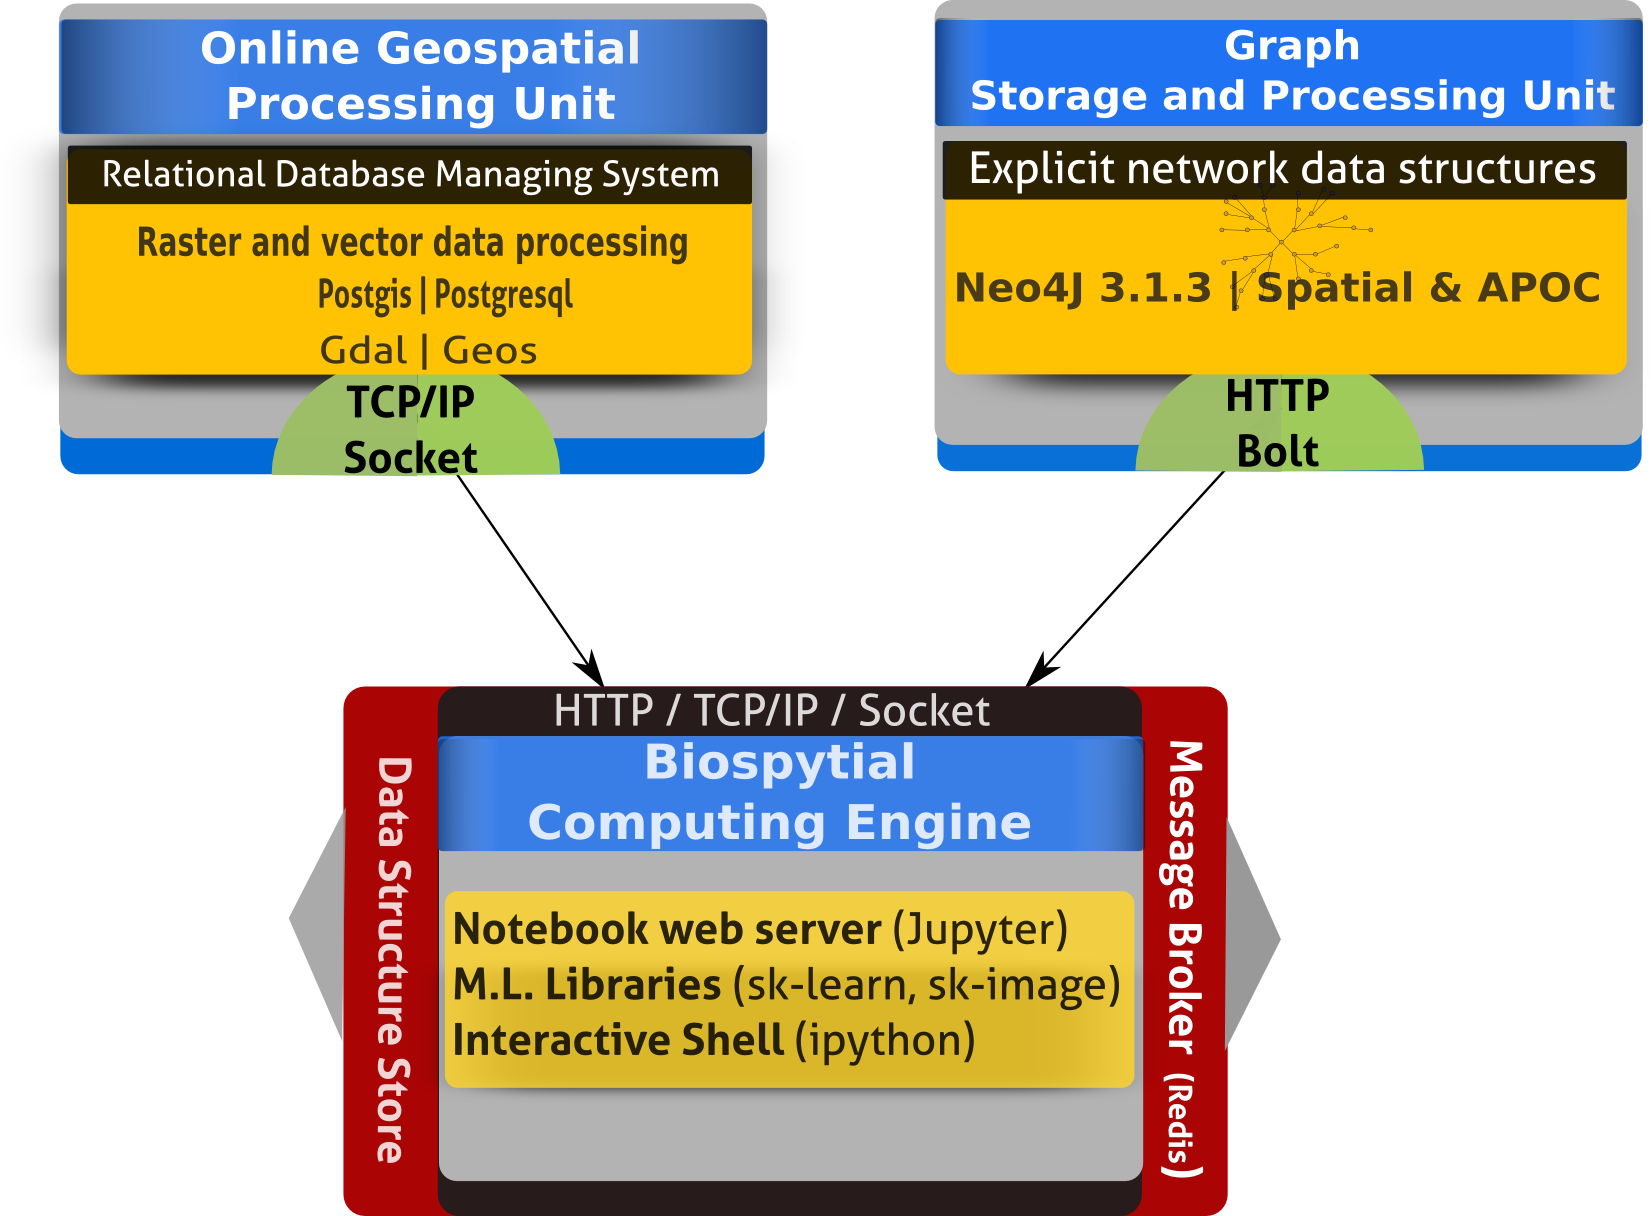
\includegraphics[scale=0.4]{biospytial-stack.png}
\end{frame}
\subsection{Supported Data}
\begin{frame}
\begin{block}

\end{block}
\end{frame}
\subsection{Distributed Design}
\begin{frame}
\begin{block}

\end{block}
\end{frame}
\section{Algorithms}
\begin{frame}
\begin{block}

\end{block}
\end{frame}
\subsection{Tree of Life}
\begin{frame}
\begin{block}

\end{block}
\end{frame}
\subsection{Selecting Sub Trees}
\begin{frame}
\begin{block}

\end{block}
\end{frame}
\subsection{Nested Grids}
\begin{frame}
\begin{block}

\end{block}
\end{frame}
\subsection{Monoids on Trees}
\begin{frame}
\begin{block}

\end{block}
\end{frame}
\section{Demo}
\begin{frame}{Some Demo}
\begin{block}

\end{block}
\end{frame}
\section{Code and contaners}

\begin{frame}{Code and container availability}

\end{frame}
\end{document}
